\documentclass[11pt,a4paper]{article}
\usepackage[T1]{fontenc}
\usepackage[utf8]{inputenc}
\usepackage[magyar]{babel}
\usepackage{lmodern,microtype,geometry,tabularx,longtable,booktabs,enumitem,fancyvrb}
\usepackage{tikz}
\usetikzlibrary{arrows.meta,positioning}
\usepackage[unicode,colorlinks=true,linkcolor=blue!45!black,urlcolor=blue!45!black]{hyperref}
\usepackage{xurl}
\geometry{margin=22mm}
\setlength{\parindent}{0pt}
\setlength{\parskip}{5pt}
\setlength{\emergencystretch}{3em}
\setlist{nosep,leftmargin=*}
\renewcommand{\arraystretch}{1.15}
\newcolumntype{Y}{>{\raggedright\arraybackslash}X}
\newcommand{\code}[1]{\nolinkurl{#1}}
\DefineVerbatimEnvironment{commands}{Verbatim}{fontsize=\small}
\hypersetup{pdftitle={Territory Capture -- Rendszerterv és telepítési dokumentáció}}
\begin{document}
\begin{center}
{\LARGE\bfseries Territory Capture\par}
{\Large Rendszerterv és telepítési dokumentáció\par}
Szoftverarchitektúrák (VIAUMA21)\par
Dokumentumverzió: 1.0\quad Állapotfelvétel: 2026. november 27.\par
Vizsgált forrásverzió: \code{268cd38}
\end{center}
\setcounter{tocdepth}{1}
\tableofcontents
\newpage

\section{Bevezetés és a dokumentum hatóköre}
A Territory Capture helyi, körökre osztott területfoglaló játék. Kettő--négy résztvevő ugyanabban a böngészőben, egymást váltva játszik egy hexagonális pályán; gépi ellenfelek is beállíthatók. A játékos a területe színének megváltoztatásával foglal el új mezőket. A cél a legnagyobb terület megszerzése.

Ez a dokumentum a rendszer felépítését, tervezési döntéseit, adatmodelljét, működését, tesztelését és telepítését ismerteti. Fejlesztőknek és a rendszer műszaki értékelőinek szól; a futtatási és használati részek a bemutatást és az üzemeltetést is támogatják. A funkciók részletes elfogadási alapja a külön \code{docs/specification.tex} követelményspecifikáció. Ez a rendszerterv nem helyettesíti azt.

A szerkezet a házifeladat-útmutató 4.1. és 5.2. pontját követi: architekturális tervet, részletes réteg- és funkcióleírást, magyarázó ábrákat, telepítési útmutatót, befejezést és továbbfejlesztési lehetőségeket tartalmaz. A statikus, dinamikus és telepítési nézetet a dokumentálási előadás szempontjai alapján külön kezeli. A jelenlegi implementáció korlátait a \ref{sec:limits}. szakasz rögzíti; a tervezett viselkedést nem tekinti automatikusan megvalósítottnak.

\section{Rendszerkörnyezet és funkcionális áttekintés}
\subsection{Platform és rendszerhatár}
Az alkalmazás C\# nyelven, .NET~10 platformon, standalone Blazor WebAssembly alkalmazásként működik. A játéklogika a böngészőben fut, az aktív állapotot a controller a böngésző memóriájában tartja. A statikus HTTP(S)-kiszolgáló az alkalmazás fájljait szolgálja ki; nem játékvezérlő backend. Nincs központi adatbázis, bejelentkezés vagy hálózati többjátékos mód. A böngésző JavaScript-interoppal elért \code{localStorage} tárolja az egyetlen mentést.

A célkörnyezet asztali Chrome és Edge, legalább 1280~$\times$~720-as ablakmérettel. Ez célplatform-meghatározás, nem a böngészőkben elvégzett elfogadási teszt igazolása. A felhasználónak nem kell .NET SDK-t telepítenie; az SDK a forrás fordításához szükséges.

\begin{figure}[htbp]\centering

\begin{tikzpicture}[font=\small,box/.style={draw,rounded corners,align=center,text width=36mm,minimum height=13mm},a/.style={-{Latex}}]
\node[box] (host) at (0,0) {Statikus HTTP(S)-host\\HTML, CSS, .NET/WASM};
\node[box] (browser) at (5.6,0) {Böngésző\\UI, controller, szabályok};
\node[box] (storage) at (11.2,0) {Böngésző localStorage\\egy JSON-pillanatkép};
\draw[a] (host)--node[above]{fájlletöltés}(browser);
\draw[Latex-Latex] (browser)--node[above]{JS interop}(storage);
\end{tikzpicture}
\caption{Telepítési és futtatási környezet. A böngészőn belüli modulok nem külön szerverek.}
\end{figure}

\subsection{Követelmények és megvalósító komponensek}
\begin{tabularx}{\linewidth}{@{}lYY@{}}\toprule
Azonosító & Funkció & Megvalósítás fő helye \\\midrule
F01 / UC01 & Játszma indítása, résztvevők & Web beállítások; Application indítás; Rules generálás.\\
F02 / UC02 & Színváltás, teljes láncfoglalás & Rules: \code{ApplyMove}.\\
F03 / UC02 & Körsorrend, lépésengedélyezés & Rules következő állapot; Application parancsfogadás.\\
F04 / UC03 & Automatikus gépi kör & Infrastructure stratégia; Application gépi ciklus.\\
F05 / UC02 & Pálya, tulajdonos, pontszám & Web SVG; Application view; Rules összesítés.\\
F06 / UC04--05 & Győzelem, döntetlen, új játék & Rules befejezés; Application reset; Web eredmény.\\
F07 / UC06 & Mentés emberi körben & Application feltételek; Infrastructure JSON és tárolás.\\
F08 / UC07 & Mentés folytatása & Infrastructure beolvasás; Rules validálás; Application visszaállítás.\\\bottomrule
\end{tabularx}

A pálya 12 oszlopból és 10 sorból, összesen 120 mezőből áll. A hat szín azonosítói rögzítettek: Red=0, Orange=1, Yellow=2, Green=3, Blue=4, Purple=5. Legalább egy emberi játékos szükséges. Egy lépés a teljes saját terület átszínezése és az új színnel élmentén elérhető összes semleges mező elfoglalása. Más játékos aktuális színe és a saját aktuális szín nem választható. Nulla nyereségű szabályos lépés is átadja a kört. A játék semleges mező hiányában ér véget; azonos maximális pontszám esetén döntetlen az eredmény.

\section{Architekturális nézetek és döntések}
\subsection{Logikai rétegek és projektfüggőségek}
A rendszer legalább három logikai réteget különít el: megjelenítés, alkalmazásvezérlés és játéklogika. Ezeket infrastruktúra-adapter és közös Contracts assembly egészíti ki. A projekt és a réteg fogalma nem azonos: öt produkciós projekt van, de a Contracts nem külön üzleti feldolgozási lépcső.

\begin{figure}[htbp]\centering
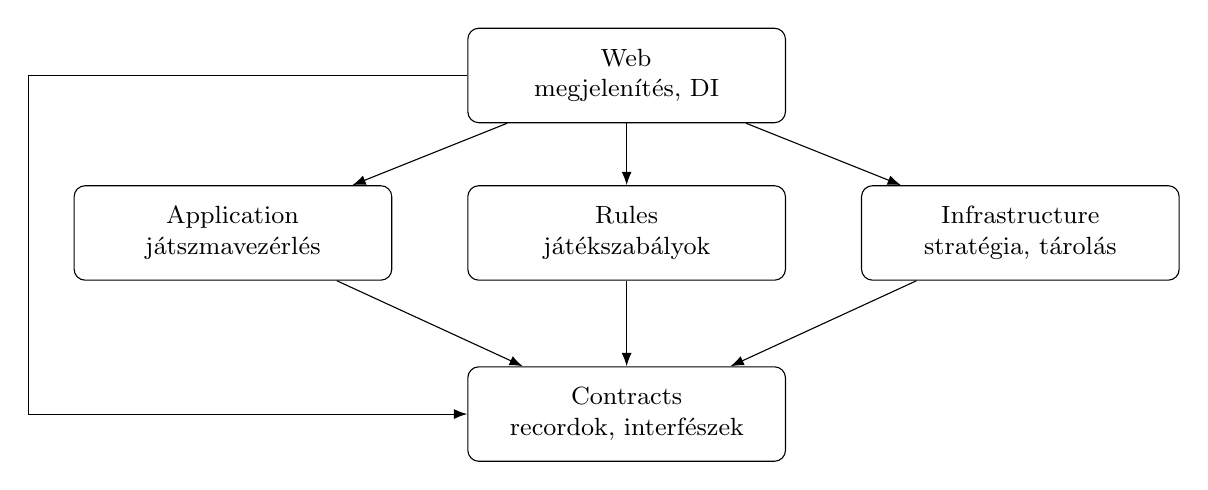
\begin{tikzpicture}[font=\small,box/.style={draw,rounded corners,align=center,text width=38mm,minimum height=12mm},a/.style={-{Latex}}]
\node[box] (web) at (0,0) {Web\\megjelenítés, DI};
\node[box] (app) at (-5,-2) {Application\\játszmavezérlés};
\node[box] (rules) at (0,-2) {Rules\\játékszabályok};
\node[box] (infra) at (5,-2) {Infrastructure\\stratégia, tárolás};
\node[box] (contracts) at (0,-4.3) {Contracts\\recordok, interfészek};
\draw[a] (web)--(app);\draw[a] (web)--(rules);\draw[a] (web)--(infra);
\draw[a] (web.west)--(-7.6,0)--(-7.6,-4.3)--(contracts.west);
\draw[a] (app)--(contracts);\draw[a] (rules)--(contracts);\draw[a] (infra)--(contracts);
\end{tikzpicture}
\caption{Fordítási függőségek. A nyíl a hivatkozó projektből a hivatkozott projektbe mutat.}
\label{fig:dependencies}
\end{figure}

A Web azért hivatkozik a konkrét implementációs projektekre is, mert a \code{Program.cs} a composition root: itt történik az interfészek és implementációk DI-regisztrációja. Az Application a \code{IGameRules}, \code{IComputerStrategy} és \code{IGameSaveStore} interfészeket ismeri a Contracts projekten keresztül, nem a Rules és Infrastructure konkrét osztályait. A fordítási gráf ezért eltér a futásidejű hívások útjától.

\begin{tabularx}{\linewidth}{@{}lY@{}}\toprule
Projekt & Felelősség és fontos fájlok \\\midrule
Contracts & \code{RulesContracts.cs}: állapot és szabályinterfész; \code{ApplicationContracts.cs}: view és facade; \code{PersistenceContracts.cs}: stratégia, snapshot, tárolási port.\\
Rules & A \code{GameRules} partial osztály fájljai: Generation, Moves, Summary és Validation. A \code{GameRules.cs} az interfész-megvalósítást deklarálja. A fájlbontás egy osztályt rendez témákra, nem külön szolgáltatásokat hoz létre.\\
Application & \code{GameController.cs}: az aktív session, parancsfogadás, view-előállítás, gépi ciklus és mentés/folytatás vezérlése.\\
Infrastructure & \code{GreedyComputerStrategy.cs}; \code{BrowserGameSaveStore.cs}; az aktív \code{GameSnapshotJsonCodec.cs}; DI-extension. A külön \code{GameSnapshotCodec.cs} a jelenlegi produkciós tárolási útvonalon nincs használatban.\\
Web & \code{App.razor}: képernyők, eseménykezelők és SVG; \code{Program.cs}: DI; \code{wwwroot}: HTML, CSS és statikus tartalom.\\\bottomrule
\end{tabularx}

\subsection{Miért ez az architektúra?}
\textbf{Rétegezés és interfészek.} A foglalási algoritmusnak nincs szüksége böngészőre, a UI-nak pedig nem kell ismernie a bejárás részleteit. Az elkülönítés lehetővé teszi a szabályok és a vezérlés célzott tesztelését, és csökkenti egy módosítás hatását. Az interfészeken átadott függőségek a dependency inversion elvét követik. A többlet néhány kis interfész és adatobjektum; ennél a méretnél külön hálózati szolgáltatások működtetése nem lenne indokolt.

\textbf{Standalone WebAssembly.} Az egygépes, körökre osztott játék nem igényel központi állapotot. A választás egyszerű statikus telepítést és telepítés nélküli böngészős használatot ad. Korlátja, hogy a mentés böngészőhöz és originhez kötött, az állapot pedig kliensoldalon módosítható. A megoldás nem nyújt többeszközös szinkronizálást vagy szerveroldali csalásvédelmet.

\textbf{Facade: \code{IGameController}.} A UI egyetlen belépési ponton indít játékot, választ színt, ment és folytat. A \code{GameController} fogja össze a szabályokat, stratégiát és tárolást, így a komponensnek nem kell ezek hívási sorrendjét ismernie. Ez nem MVC-controller: Blazor-komponensből hívott alkalmazásszolgáltatás.

\textbf{Strategy: \code{IComputerStrategy}.} A színválasztási döntés elkülönül a lépés végrehajtásától. Jelenleg egy mohó implementáció van; más döntési algoritmus azonos interfész mögé helyezhető. A közös \code{ApplyMove} használata biztosítja, hogy a szimuláció és a tényleges foglalás ugyanazt a szabályt alkalmazza.

\textbf{Tárolási adapter.} A \code{BrowserGameSaveStore} valósítja meg a \code{IGameSaveStore} portot. Az alkalmazásréteg snapshotot ad át, nem JavaScript-hívásokat hajt végre. A JSON-formátum és a böngészős I/O külön osztályban van, ezért a codec szövegekkel, az adapter pedig helyettesített JS runtime-mal tesztelhető. Ehhez az egyetlen mentési helyhez egy általános Repository vagy ORM további hasznos viselkedést nem adna.

\textbf{Immutable állapot és változásértesítés.} Az állapot recordokból és \code{ImmutableArray} gyűjteményekből áll. Egy lépés új állapotot ad vissza; a korábbi állapot megmarad a szimulációhoz vagy mentési snapshothoz. A UI a \code{Changed} eseményre újrarenderel. Ez eseményalapú értesítés, nem event sourcing: nincs eltárolt eseménynapló.

\section{Adatmodell és algoritmusok}
\subsection{Állapotmodell}
\begin{figure}[htbp]\centering
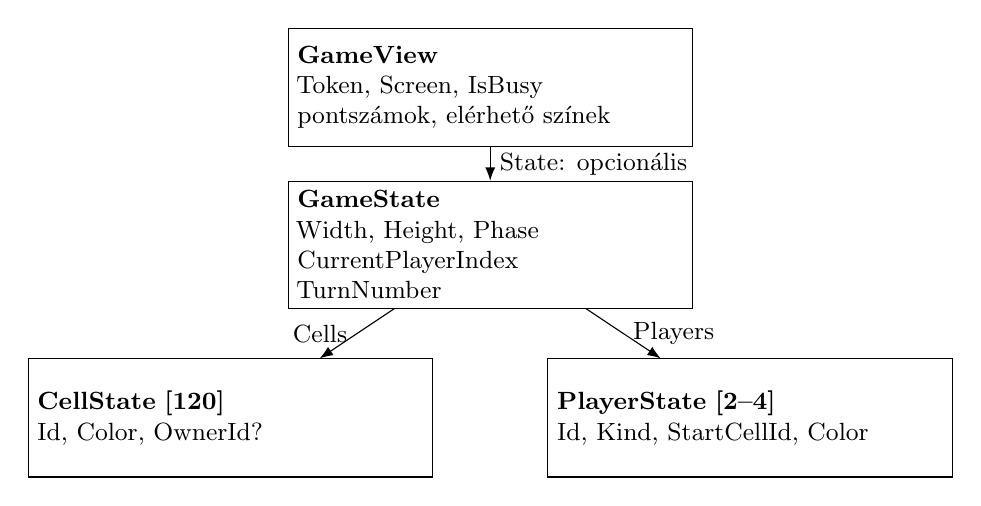
\begin{tikzpicture}[font=\small,box/.style={draw,align=left,text width=49mm,minimum height=15mm},a/.style={-{Latex}}]
\node[box] (view) at (0,0) {\textbf{GameView}\\Token, Screen, IsBusy\\pontszámok, elérhető színek};
\node[box] (state) at (0,-2) {\textbf{GameState}\\Width, Height, Phase\\CurrentPlayerIndex\\TurnNumber};
\node[box] (cells) at (-3.3,-4.2) {\textbf{CellState [120]}\\Id, Color, OwnerId?};
\node[box] (players) at (3.3,-4.2) {\textbf{PlayerState [2--4]}\\Id, Kind, StartCellId, Color};
\draw[a] (view)--node[right]{State: opcionális}(state);
\draw[a] (state)--node[left]{Cells}(cells);
\draw[a] (state)--node[right]{Players}(players);
\end{tikzpicture}
\caption{Az adatmodell fő kapcsolatai; a nyilak adatmező-hivatkozások, nem öröklések.}
\end{figure}

A mező színe és tulajdonosa külön adat. Azonos szín nem jelent azonos tulajdonost, egy semleges mezőnek pedig nincs tulajdonosa. A \code{CellState.Id = row * 12 + column}; a játékosazonosító a résztvevőlista indexe. A pontszám nem külön módosított számláló: a Rules a tulajdonosazonosítók megszámolásával számítja. A \code{GameView} ennek megjelenítési vetületét tartalmazza; Setup állapotban nincs benne \code{GameState}.

A \code{ViewToken} sessionazonosítót és revisiont tartalmaz. Új játék új sessiont kap; a közzétett állapotváltozások revisionje növekszik. A controller a színválasztás és mentés tokenjét a jelenlegivel hasonlítja össze. Ez az elavult parancsok kiszűrését szolgálja, nem felhasználó-hitelesítés.

\subsection{Generálás és hexszomszédság}
A \code{Create} ellenőrzi a résztvevőket, seedelt \code{Random} példánnyal megkeveri a palettát és eltérő kezdőszíneket rendel a játékosokhoz, majd véletlenszerűen színezi a táblát. A kezdőcellák színét a játékosokéhoz igazítja, végül befoglalja a kezdőponttal összefüggő azonos színű komponenst. A kezdőmezőket a jelenlegi kód játékosszám szerint választja: kettőnél \code{[0,119]}, háromnál \code{[0,11,119]}, négynél \code{[0,11,108,119]}. Ez a konkrét sorrend eltér a korábbi munkaterv sorrendjétől; a modell validálása is ezeket a kódbeli pozíciókat várja.

A koordinátarendszer pointy-top, odd-r: a páratlan sorok fél mezőszélességgel jobbra tolódnak. Minden mező vízszintes szomszédai $(c-1,r)$ és $(c+1,r)$. Páros sorban a két szomszédos sor oszlopai $c-1,c$, páratlan sorban $c,c+1$. A határ ellenőrzése mindkét koordinátán történik, nincs körbeérés. A UI ugyanilyen eltolással rajzol, de a foglalást a Rules végzi.

\subsection{Foglalás és összesítés}
Az \code{ApplyMove} először validálja az állapotot, ellenőrzi a fázist, játékost, körsorrendet, színt és a körszámláló túlcsordulását. Az állapot immutable gyűjteményeiből helyi buildert készít. A saját mezőket átszínezi, majd az összes saját mezőt egy BFS-sorba helyezi. A bejárás kizárólag semleges, választott színű mezőt foglalhat el és tehet a sorba. Így nem csak a kezdőpont környéke, hanem a teljes terület határa számít.

Siker esetén a \code{CapturedCount} az újonnan megszerzett mezők száma. A körszám eggyel nő, a következő játékos indexe modulo résztvevőszám számítódik. Ha nincs semleges mező, a fázis Finished, és az utolsó lépő indexe marad meg. Az eredeti állapot nem módosul. A \code{Summarize} visszaadja a pontszámokat és semleges mezők számát; győztesazonosítókat csak befejezett játékhoz ad.

\subsection{Gépi stratégia és költség}
A \code{GreedyComputerStrategy} minden szabályos színre meghívja a közös szabálymotor \code{ApplyMove} műveletét. A legnagyobb \code{CapturedCount} értékű színt választja; döntetlennél a numerikus palettasorrend dönt. Nulla nyereségnél is szabályos lépést választ. A szimulált utódállapotokat nem telepíti az aktív játékba; azt a controller végzi a kiválasztott színnel.

A hexgráf csúcsainak foka legfeljebb hat, ezért egy BFS költsége $O(N)$. A teljes validálás és összesítés játékosonként is vizsgálhatja a táblát, így egy lépés költsége $O(PN)$, a mohó választásé $O(KPN)$; $P\leq4$, $K\leq4$, $N=120$. A kis tábla miatt nincs szükség párhuzamos bejárásra vagy háttérszálra. A költségbecslés algoritmikus korlát, nem futásidőmérés.

\section{Futásidejű működés}
\subsection{Emberi lépés és UI-frissítés}
\begin{figure}[htbp]\centering
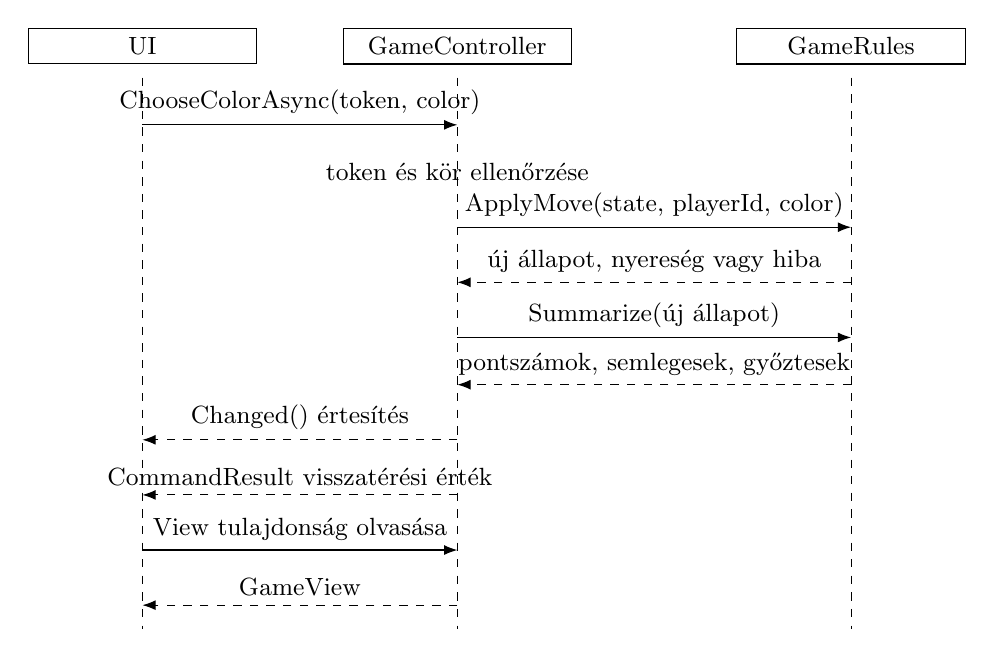
\begin{tikzpicture}[font=\small,a/.style={-{Latex}},reply/.style={dashed,-{Latex}}]
\foreach \x/\name in {0/UI,4/GameController,9/GameRules}{
\node[draw,minimum width=29mm] at (\x,0) {\name};
\draw[dashed] (\x,-0.4)--(\x,-7.4);}
\draw[a] (0,-1)--node[above]{ChooseColorAsync(token, color)}(4,-1);
\node[align=center] at (4,-1.6) {token és kör ellenőrzése};
\draw[a] (4,-2.3)--node[above]{ApplyMove(state, playerId, color)}(9,-2.3);
\draw[reply] (9,-3)--node[above]{új állapot, nyereség vagy hiba}(4,-3);
\draw[a] (4,-3.7)--node[above]{Summarize(új állapot)}(9,-3.7);
\draw[reply] (9,-4.3)--node[above]{pontszámok, semlegesek, győztesek}(4,-4.3);
\draw[reply] (4,-5)--node[above]{Changed() értesítés}(0,-5);
\draw[reply] (4,-5.7)--node[above]{CommandResult visszatérési érték}(0,-5.7);
\draw[a] (0,-6.4)--node[above]{View tulajdonság olvasása}(4,-6.4);
\draw[reply] (4,-7.1)--node[above]{GameView}(0,-7.1);
\end{tikzpicture}
\caption{Sikeres emberi lépés fő hívásai; a view olvasása az újrarendereléskor történik. A hibás parancs nem hajt végre játékbeli lépést.}
\end{figure}

Az UI a facade metódusait hívja. A controller a \code{BuildGameView} segítségével számítja a megjelenítési adatokat; a Game képernyőn, emberi körben, más művelet hiányában a \code{LegalColors} műveletet is meghívja. A \code{Changed} paraméter nélküli esemény, a UI az újrarendereléskor a \code{View} tulajdonságot olvassa. A parancs külön \code{CommandResult} eredményt ad vissza. A komponens \code{Changed} eseményre \code{InvokeAsync(StateHasChanged)} hívással frissít, és megszűnésekor leiratkozik az eseményről. Jelenleg a felület egyetlen \code{App.razor} fájlban tartalmazza a beállítási, játék- és eredménynézetet.

\subsection{Gépi körök és új játék}
A \code{CheckAndStartComputerRunner} gépi játékosnál aszinkron ciklust indít. A ciklus \code{Task.Delay(1, token)} hívással átadja a végrehajtást, meghívja a stratégiát, majd a szabálymotort és közzéteszi az új állapotot. Emberi körnél vagy befejezett játékban megáll. Ez kooperatív aszinkron működés, nem párhuzamos számítás.

Új játék kezdeményezésekor a controller megszakítja az aktuális megszakítási tokent és új Setup view-t közöl új sessionazonosítóval. A gépi eredmény alkalmazása előtt a megszakítás jelzését és a session egyezését is ellenőrzi. Az új játék nem hív tárolótörlést. A gépi körben a view szabályos emberi színlistája üres; az \code{IsBusy} önmagában nem jelenti azt, hogy gépi kör van. A kivételt a controller háttérhibaként jelzi; az összes hibautat érintő garanciák korlátait a \ref{sec:limits}. szakasz írja le.

\subsection{Mentés, formátum és folytatás}
A mentés csak futó játék emberi körében, két művelet között engedélyezett. A controller rögzíti a snapshotot és a view-ban jelzi a folyamatban lévő mentést. A tárolási adapter a \code{GameSnapshotJsonCodec} segítségével teljesen előállítja a JSON-t, majd egyetlen \code{localStorage.setItem} hívással lecseréli a régi értéket; nem törli előzetesen. A kulcs \code{territory-capture.save.v1}, a formátum verziója 1.

A snapshot mezői: \code{version}, \code{state}; azon belül \code{width}, \code{height}, \code{cells}, \code{players}, \code{currentPlayerIndex}, \code{turnNumber}, \code{phase}. Minden cella \code{id}, \code{color}, \code{ownerId} mezőt tartalmaz; minden játékos \code{id}, \code{kind}, \code{startCellId}, \code{color} mezőt. Az enumok numerikusak. A kötelező \code{ownerId} értéke lehet JSON null. Pontszám, view-token, busy flag és függőségek nem kerülnek a mentésbe.

A codec külön DTO-kat és source-generated JSON-metaadatokat használ, így a trimmed WebAssembly publish nem a domain recordok reflection alapú szerializációjától függ. A felső mérethatár 256 KiB UTF-8 adat. A verzió, kötelező mezők, adattípusok és enumértékek ellenőrzése a codec feladata; a tábla szemantikai konzisztenciáját a \code{GameRules.Validate} vizsgálja. A böngészős hozzáférési hibát az adapter képezi \code{StoreError.Unavailable} értékre; ez nem a codec eredménye és nem sikeres mentés.

Folytatáskor a controller betölti a jelölt snapshotot, a szabálymotorral validálja, majd csak futó, emberi körben levő állapotot fogad el. Nem generálja újra a táblát. Az aktív pontszámok az állapotból újraszámolódnak. A localStorage írás megtörténhet akkor is, ha egy későbbi megszakítás miatt a hívó már nem kap sikeres visszajelzést; a megszakítás nem adatbázis-tranzakciós rollback.

\section{Validálás, biztonság és ismert korlátok}
\subsection{Validálási határok}
A Rules ellenőrzi a 120 cellát, sorrendjüket, azonosítóikat, a játékosokat és kezdőmezőket, a színek egyediségét, a tulajdonosok létezését és színegyezését, a területek összefüggőségét, a befoglalás lezártságát és a fázis/semleges mezők konzisztenciáját. A codec által olvasható JSON még nem feltétlenül érvényes játékállapot. Az Application külön ellenőrzi, hogy az adott parancs az aktuális képernyőn és körben engedélyezett-e.

A rendszer helyi játék: nincs felhasználói fiók és nem kezel központi jogosultságot. Adatbázis hiányában SQL injection útvonal sincs. A kliensoldali mentés nem titkosított és nem hitelesített; saját böngészőadatainak manipulálását a rendszer nem tudja általánosan megakadályozni. Nyilvános telepítéshez HTTPS szükséges. A játékadat szöveges megjelenítése Blazor markupban történik; nincs felhasználói HTML-import.

\subsection{Jelenlegi implementációs korlátok}\label{sec:limits}
Az alábbiak a vizsgált forrás állapotára vonatkoznak, nem a kívánt működés átértelmezései:
\begin{enumerate}
\item A \code{ResumeAsync} minden tárolási hibát \code{MissingSave} eredményre képez, noha az adattárolási réteg külön hibakóddal jelzi a hiányzó mentést, a sérült adatot, az ismeretlen verziót és a hozzáférési hibát. A UI hibatérképe részletesebb a jelenleg továbbított információnál.
\item A betöltés nem rögzít és nem ellenőriz sessionazonosítót az await után. Egy közben végrehajtott reset után késve beérkező betöltés új sessiont indíthat. Ez eltér a munkaterv késői eredményekre előírt védelmétől.
\item A UI a színválasztás és a mentés eseménykezelőjében olvassa a controller aktuális tokenjét, nem a kirajzolt view tokenjét rögzíti. A controller tokenellenőrzése létezik, de a teljes UI-oldali elavultkattintás-védelem így nem igazolt. A színválasztás visszaadott hibaeredményét a komponens nem jeleníti meg.
\item Gépi kivétel esetén a view háttérhibát tartalmaz, de a view-előállítás nem tilt minden parancsot kizárólag e hiba alapján; hibás szabályeredménynél a gépi ciklus egyszerűen megáll. Nem állítható teljes, resetig tartó hibazárolás.
\item A felület jelenleg angol szövegeket használ, a tulajdonosazonosító SVG-tooltipban olvasható, és a browser integrációs tesztekhez előírt \code{data-testid} attribútumok hiányoznak. A teljes hozzáférhetőségi és browser acceptance megfelelés nem igazolt.
\end{enumerate}
E korlátok miatt a követelmények teljes körű teljesítését önmagában a projektstruktúra vagy a unit tesztek megléte nem bizonyítja.

\section{Tesztelési terv és ellenőrzési bizonyíték}
\subsection{Szintek és tesztkörnyezet}
A .NET-tesztek xUnit alapúak, a komponensvizsgálatok bUnitot használnak. A \code{tests/TerritoryCapture.TestSupport} kézzel összeállított fixture-öket és helyettesítő függőségeket ad. A unit teszt azt a komponenst vizsgálja, amelynek a valós osztályát példányosítja; egy fake szabálymotorral futó controller-teszt nem bizonyítja a foglalási algoritmus helyességét.

\begin{tabularx}{\linewidth}{@{}lY@{}}\toprule
Tesztprojekt & Fő forgatókönyvek \\\midrule
Rules.Tests & Páros/páratlan sor szomszédai, generálás, láncfoglalás, ellenfélblokkolás, nulla nyereség, immutable bemenet, győzelem, állapotvalidálás.\\
Application.Tests & Start, emberi kör, token, reset, gépi ciklus, mentési feltételek, invalid visszatöltés; jellemzően helyettesített függőségekkel.\\
Infrastructure.Tests & Maximális teljes nyereség, palettaholtverseny, JSON round-trip, hibás/verziós adat, mérethatár, JS- és kvótahiba, cancellation.\\
Web.Tests & Controller nélküli képernyő, Debug preview, Release-ből kihagyott demoosztály. Nem teljes UI acceptance suite.\\
Integration.Tests & Jelenleg a döntetlen fixture adatainak ellenőrzése; nem teljes valós komponensintegráció.\\\bottomrule
\end{tabularx}

Két Playwright-projekt van a \code{tests/browser} alatt. Az infrastructure projekt a külön \code{BrowserHarness} publikált alkalmazásán a valódi codecet, tárolót és JS interopot vizsgálja, helyettesített játékszabályokkal. Az application projekt a valódi publikált játék emberi lépését, gépi körét és mentés/folytatás folyamatát célozza. A két suite bizonyító ereje eltér; a harness nem a telepítendő játék. A browser-tesztek parancsai és DOM-elvárásai a \code{tests/browser/README.md} fájlban találhatók.

\subsection{Reprodukálható ellenőrzés}
A repository gyökeréből:
\begin{commands}
dotnet restore TerritoryCapture.sln --locked-mode
dotnet build TerritoryCapture.sln -c Release --no-restore
dotnet test TerritoryCapture.sln -c Release --no-build --no-restore
\end{commands}
A PR-workflow ugyanezt a fő útvonalat ellenőrzi, valamint a Blazor toolchain eltérő alapértékeire locked-restore regressziós vizsgálatot végez. A CI-konfiguráció megléte nem egy konkrét távoli futás eredménye.

\textbf{Ellenőrzési állapot, 2026. november 27.:} a locked restore után futtatott \code{dotnet test TerritoryCapture.sln --configuration Release --no-restore} sikeresen lefordította a solutiont, és 128 teszteset teljesült: Rules 58, Application 16, Infrastructure 51, Integration 1, Web 2; hibás és kihagyott eset nem volt. A futtatási környezet Ubuntu 24.04, .NET SDK 10.0.402. Az eredmény a fenti komponenshatárok szerint értelmezendő, nem teljes browser acceptance igazolás. A browser suite és a Chrome/Edge kézi vizsgálat e dokumentumhoz nem került végrehajtásra. Ezeket nem tekintjük sikeresnek pusztán a tesztfájlok megléte alapján.

\subsection{Kézi elfogadási forgatókönyvek}
A publikált Release változaton ellenőrizendő:
\begin{enumerate}
\item Két emberi játékos indítása; szabályos színnel a teljes komponens foglalása, pontszám és kör frissülése.
\item Ember--gép--gép konfiguráció; a gépi körök automatikusan lefutnak, ember nem léphet közben.
\item Mentés emberi körben, lap újratöltése, folytatás; az összes cella, játékos és következő kör egyezik.
\item Új játék gépi kör közben; az előző session eredménye nem kerül az új játékba, a régi mentés megmarad.
\item Hiányzó, sérült és jövőbeli verziójú mentés; Setup használható marad, nincs részleges játékállapot. A jelenlegi összevont hibaüzenetet külön kell értékelni.
\item Teljes foglalásnál lépések tiltása, helyes győztes vagy döntetlen, a végső tábla megőrzése. Előkészített állapot csak tesztharnessben használható, nincs produkciós állapotimport.
\end{enumerate}
A jegyzőkönyvben a böngésző pontos verzióját, környezetét, elvárt és kapott eredményt, valamint az esetleges hibát kell rögzíteni.

\section{Telepítési és futtatási dokumentáció}
\subsection{Előfeltételek és konfiguráció}
A forrás fordításához a \code{global.json} által rögzített .NET SDK~10.0.402 kell; a roll-forward tiltott. A \code{Directory.Build.targets} a Blazor runtime és belső buildcsomagok verzióját 10.0.13-ra rögzíti. Ezek nem minden \code{PackageReference} verzióját jelentik: a Web és JSInterop közvetlen csomagjai 10.0.0 verziójúak. A csomagzárakat a projektek \code{packages.lock.json} fájljai tartalmazzák.

A futtatáshoz statikus HTTP(S)-host és korszerű asztali böngésző elég. A helyi kiszolgálási példához Python~3 kell. A browser-tesztekhez külön Node.js~22+, npm és Playwright Chromium szükséges; a játék futásához nem. A tesztkörnyezet telepítési lépéseit a browser README részletezi.

\subsection{Futtatás az átadott bináris csomagból}
A beadott publikált állományok használatához nem kell SDK vagy újrafordítás. Abban a könyvtárban, amely az átadott \code{index.html} fájlt és \code{_framework} alkönyvtárat tartalmazza, Python~3-mal:
\begin{commands}
python3 -m http.server 5080 --bind 127.0.0.1
\end{commands}
Ezután a \url{http://localhost:5080} címen nyitható meg a játék. A kiszolgálót a terminálban Ctrl+C állítja le. Foglalt port esetén másik szabad port választható; a mentés és folytatás során ugyanazt az origint kell használni.

\subsection{Fordítás és publikálás}
A repository gyökeréből futtatva:
\begin{commands}
dotnet --version
dotnet restore TerritoryCapture.sln --locked-mode
dotnet build TerritoryCapture.sln -c Release --no-restore
dotnet test TerritoryCapture.sln -c Release --no-build --no-restore
dotnet publish src/TerritoryCapture.Web -c Release --no-restore
\end{commands}
A telepítendő fájlok a következő könyvtárban találhatók:
\begin{commands}
src/TerritoryCapture.Web/bin/Release/net10.0/publish/wwwroot
\end{commands}
A teljes könyvtártartalmat kell átadni a kiszolgálónak, a \code{_framework} könyvtárral együtt. Nem a forrásbeli \code{wwwroot} és nem a BrowserHarness telepítendő. Helyi ellenőrzés:
\begin{commands}
python3 -m http.server 5080 --bind 127.0.0.1 \
  --directory src/TerritoryCapture.Web/bin/Release/net10.0/publish/wwwroot
\end{commands}
A cím \url{http://localhost:5080}. A HTML közvetlen, \code{file://} megnyitása nem támogatott. Nyilvános üzemhez HTTPS-képes statikus host használható. A \code{.wasm} fájlokat \code{application/wasm}, a JavaScriptet megfelelő JavaScript MIME-típussal kell kiszolgálni. A helyi Python-szerver bemutatási eszköz, nem nyilvános üzemeltetési javaslat.

\subsection{Debug és Release eltérése}
A \code{dotnet run --project src/TerritoryCapture.Web} alapértelmezett Debug/Development indítása a \code{DemoController} példányt regisztrálja. Ez előre meghatározott állapotokat ad; nem a valós játékmenet. A valódi függőségeket Release-ben, illetve Debug esetén nem Development környezetben regisztrálja a \code{Program.cs}. A végső bemutatáshoz a publikált Release változat használata indokolt.

A \code{Development/**/*.cs} fájlokat a Web projekt Release fordításkor kihagyja. A production controllerhez a \code{GameRules}, \code{GreedyComputerStrategy}, \code{BrowserGameSaveStore} és \code{GameSnapshotJsonCodec} kerül regisztrálásra. Az infrastruktúra extensionje \code{TryAdd} regisztrációkat használ; a stratégiát a Program külön is regisztrálja.

\subsection{Használat és helyi adatok}
A felületen a \emph{Participant count} és játékostípus-választók után a \emph{Start} indít. A \emph{Continue saved game} a helyi mentést tölti be. Emberi körben a megjelenő színgombokkal lehet lépni, a \emph{Save} ment, a \emph{New game / Setup} visszatér a beállításokhoz. Az eredményképernyőn a végső tábla, pontszámok és győztesek látszanak.

A mentés az originhez (protokoll, host, port) és a böngészőprofilhoz kötött. Másik port, másik böngésző vagy HTTP-ről HTTPS-re váltás más tárolóterületet jelent. Az oldal újratöltésekor a nem mentett lépések elvesznek; a mentett állás külön folytatható. A böngészőadatok törlése törli a mentést is. A rendszerben nincs export/import, automatikus mentés vagy központi backup. Frissítéskor az origin és az 1-es JSON-séma kompatibilitását meg kell őrizni, vagy külön migrációt kell tervezni.

Gyökérútvonalra történő telepítést feltételez a \code{wwwroot/index.html} fájl \code{<base href="/">} beállítása. Alkönyvtáras telepítéshez a base útvonalat és a host beállításait össze kell hangolni. Hiányzó statikus assetnél a böngésző Network panelje, illetve konzolja segít; storage-hibánál a böngésző tárolási engedélyeit és kvótáját kell ellenőrizni.

\subsection{Beadandó csomag}
A házifeladat-útmutató szerinti csomagnak külön azonosíthatóan tartalmaznia kell a követelményspecifikációt, ezt a rendszertervet és telepítési leírást, valamint a megvalósított rendszer forrását és publikált bináris/statikus állományait. A PDF-ek elkészítése önmagában nem helyettesíti a futtatható rendszer átadását. E dokumentum fordítása a repository gyökeréből:
\begin{commands}
latexmk -cd -pdf -interaction=nonstopmode -halt-on-error \
  -outdir=build docs/rendszerterv.tex
\end{commands}
Az eredmény \code{docs/build/rendszerterv.pdf}. A specifikáció külön fordítható a meglévő \code{make -C docs} paranccsal. A bemutatást az útmutató szerint a feltöltés előtt kell megtartani, előzetesen egyeztetett időpontban.

\section{Továbbfejlesztési lehetőségek és befejezés}
Elsőbbséget élvez a \ref{sec:limits}. szakaszban felsorolt korlátok rendezése és a valós komponensekkel végzett elfogadási vizsgálat. Ezután a UI kisebb komponensekre bontása, látható tulajdonosjelölések és jobb billentyűzetes használat javítaná a karbantarthatóságot és hozzáférhetőséget. Új stratégia az \code{IComputerStrategy} mögött illeszthető be. Több mentési hely vagy export a tárolási szerződés és UI bővítését, sémafrissítés verziózott migrációt igényel.

A hálózati játék már lényeges architekturális változás: szerveroldali hiteles állapotot, játékosazonosítást és konkurens parancskezelést kívánna. Nem tekinthető pusztán a localStorage-adapter cseréjének.

A választott rétegezés a helyi játék igényeihez igazodik: a szabályok függetlenek a felülettől és tárolástól, a facade összefogja az alkalmazásműveleteket, a Strategy külön kezeli a gépi döntést. A dokumentált függőségek és a tesztelési határok egyértelművé teszik, mely komponens milyen működésért felel és mely állítások igényelnek még integrációs bizonyítékot.

\section*{Fogalomtár}\addcontentsline{toc}{section}{Fogalomtár}
\begin{tabularx}{\linewidth}{@{}lY@{}}\toprule
Fogalom & Jelentés ebben a rendszerben \\\midrule
Session & Egy aktív játszma vezérlési élettartama, saját azonosítóval.\\
Snapshot & A folytatáshoz szükséges teljes játékállapot egy pillanatban.\\
DTO & A JSON-formátumhoz használt külön adatobjektum; nem a UI view-ja.\\
Composition root & A konkrét implementációkat összekötő DI-konfiguráció, itt a Program.\\
BFS & Sor alapú szélességi bejárás a hexgráf összefüggő részeinek keresésére.\\
Origin & A böngészős tárolót elválasztó protokoll--host--port hármas.\\
Fixture / test double & Előre ismert tesztadat / egy függőség tesztbeli helyettesítője.\\\bottomrule
\end{tabularx}

\section*{Hivatkozások}\addcontentsline{toc}{section}{Hivatkozások}
\begin{enumerate}
\item \emph{Szoftverarchitektúrák (VIAUMA21) házi feladat útmutató}, 2026. Helyi forrás: \code{HaziFeladatHallgatoiUtmutato_2026.pdf}, különösen 4.1--4.2. és 5.2--5.3. pont.
\item \emph{Szoftverarchitektúrák -- Dokumentálás}, 2026. Helyi forrás: \code{09.eloadas2026_Dokumentalas.pdf}; statikus/dinamikus nézetek, algoritmusok, tesztelés és telepítés dokumentálása.
\item A projekt követelményspecifikációja: \code{docs/specification.tex}.
\item A vizsgált implementáció: \code{src/TerritoryCapture.*}; tesztek: \code{tests}; toolchain: \code{global.json}, \code{Directory.Build.props}, \code{Directory.Build.targets}.
\end{enumerate}
\end{document}
